% GNUPLOT: LaTeX picture with Postscript
\begingroup
  % Encoding inside the plot.  In the header of your document, this encoding
  % should to defined, e.g., by using
  % \usepackage[latin1,<other encodings>]{inputenc}
  \inputencoding{latin1}%
  \makeatletter
  \providecommand\color[2][]{%
    \GenericError{(gnuplot) \space\space\space\@spaces}{%
      Package color not loaded in conjunction with
      terminal option `colourtext'%
    }{See the gnuplot documentation for explanation.%
    }{Either use 'blacktext' in gnuplot or load the package
      color.sty in LaTeX.}%
    \renewcommand\color[2][]{}%
  }%
  \providecommand\includegraphics[2][]{%
    \GenericError{(gnuplot) \space\space\space\@spaces}{%
      Package graphicx or graphics not loaded%
    }{See the gnuplot documentation for explanation.%
    }{The gnuplot epslatex terminal needs graphicx.sty or graphics.sty.}%
    \renewcommand\includegraphics[2][]{}%
  }%
  \providecommand\rotatebox[2]{#2}%
  \@ifundefined{ifGPcolor}{%
    \newif\ifGPcolor
    \GPcolortrue
  }{}%
  \@ifundefined{ifGPblacktext}{%
    \newif\ifGPblacktext
    \GPblacktexttrue
  }{}%
  % define a \g@addto@macro without @ in the name:
  \let\gplgaddtomacro\g@addto@macro
  % define empty templates for all commands taking text:
  \gdef\gplbacktext{}%
  \gdef\gplfronttext{}%
  \makeatother
  \ifGPblacktext
    % no textcolor at all
    \def\colorrgb#1{}%
    \def\colorgray#1{}%
  \else
    % gray or color?
    \ifGPcolor
      \def\colorrgb#1{\color[rgb]{#1}}%
      \def\colorgray#1{\color[gray]{#1}}%
      \expandafter\def\csname LTw\endcsname{\color{white}}%
      \expandafter\def\csname LTb\endcsname{\color{black}}%
      \expandafter\def\csname LTa\endcsname{\color{black}}%
      \expandafter\def\csname LT0\endcsname{\color[rgb]{1,0,0}}%
      \expandafter\def\csname LT1\endcsname{\color[rgb]{0,1,0}}%
      \expandafter\def\csname LT2\endcsname{\color[rgb]{0,0,1}}%
      \expandafter\def\csname LT3\endcsname{\color[rgb]{1,0,1}}%
      \expandafter\def\csname LT4\endcsname{\color[rgb]{0,1,1}}%
      \expandafter\def\csname LT5\endcsname{\color[rgb]{1,1,0}}%
      \expandafter\def\csname LT6\endcsname{\color[rgb]{0,0,0}}%
      \expandafter\def\csname LT7\endcsname{\color[rgb]{1,0.3,0}}%
      \expandafter\def\csname LT8\endcsname{\color[rgb]{0.5,0.5,0.5}}%
    \else
      % gray
      \def\colorrgb#1{\color{black}}%
      \def\colorgray#1{\color[gray]{#1}}%
      \expandafter\def\csname LTw\endcsname{\color{white}}%
      \expandafter\def\csname LTb\endcsname{\color{black}}%
      \expandafter\def\csname LTa\endcsname{\color{black}}%
      \expandafter\def\csname LT0\endcsname{\color{black}}%
      \expandafter\def\csname LT1\endcsname{\color{black}}%
      \expandafter\def\csname LT2\endcsname{\color{black}}%
      \expandafter\def\csname LT3\endcsname{\color{black}}%
      \expandafter\def\csname LT4\endcsname{\color{black}}%
      \expandafter\def\csname LT5\endcsname{\color{black}}%
      \expandafter\def\csname LT6\endcsname{\color{black}}%
      \expandafter\def\csname LT7\endcsname{\color{black}}%
      \expandafter\def\csname LT8\endcsname{\color{black}}%
    \fi
  \fi
    \setlength{\unitlength}{0.0500bp}%
    \ifx\gptboxheight\undefined%
      \newlength{\gptboxheight}%
      \newlength{\gptboxwidth}%
      \newsavebox{\gptboxtext}%
    \fi%
    \setlength{\fboxrule}{0.5pt}%
    \setlength{\fboxsep}{1pt}%
\begin{picture}(7488.00,4896.00)%
    \gplgaddtomacro\gplbacktext{%
      \csname LTb\endcsname%%
      \put(396,594){\makebox(0,0){\fontsize{8.5}{8.5}\selectfont{4}}}%
      \put(396,1005){\makebox(0,0){\fontsize{8.5}{8.5}\selectfont{6}}}%
      \put(396,1416){\makebox(0,0){\fontsize{8.5}{8.5}\selectfont{8}}}%
      \put(396,1827){\makebox(0,0){\fontsize{8.5}{8.5}\selectfont{10}}}%
      \put(396,2238){\makebox(0,0){\fontsize{8.5}{8.5}\selectfont{12}}}%
      \put(396,2649){\makebox(0,0){\fontsize{8.5}{8.5}\selectfont{14}}}%
      \put(396,3060){\makebox(0,0){\fontsize{8.5}{8.5}\selectfont{16}}}%
      \put(396,3471){\makebox(0,0){\fontsize{8.5}{8.5}\selectfont{18}}}%
      \put(396,3882){\makebox(0,0){\fontsize{8.5}{8.5}\selectfont{20}}}%
      \put(396,4293){\makebox(0,0){\fontsize{8.5}{8.5}\selectfont{22}}}%
      \put(672,396){\rotatebox{45}{\makebox(0,0)[l]{\strut{}\fontsize{5.5}{5.5}\selectfont{8,1}}}}%
      \put(883,396){\rotatebox{45}{\makebox(0,0)[l]{\strut{}\fontsize{5.5}{5.5}\selectfont{7,2}}}}%
      \put(1093,396){\rotatebox{45}{\makebox(0,0)[l]{\strut{}\fontsize{5.5}{5.5}\selectfont{6,3}}}}%
      \put(1304,396){\rotatebox{45}{\makebox(0,0)[l]{\strut{}\fontsize{5.5}{5.5}\selectfont{5,4}}}}%
      \put(1514,396){\rotatebox{45}{\makebox(0,0)[l]{\strut{}\fontsize{5.5}{5.5}\selectfont{4,5}}}}%
      \put(1725,396){\rotatebox{45}{\makebox(0,0)[l]{\strut{}\fontsize{5.5}{5.5}\selectfont{3,6}}}}%
      \put(1935,396){\rotatebox{45}{\makebox(0,0)[l]{\strut{}\fontsize{5.5}{5.5}\selectfont{2,7}}}}%
      \put(2146,396){\rotatebox{45}{\makebox(0,0)[l]{\strut{}\fontsize{5.5}{5.5}\selectfont{1,8}}}}%
      \put(2356,396){\rotatebox{45}{\makebox(0,0)[l]{\strut{}\fontsize{5.5}{5.5}\selectfont{8,0}}}}%
      \put(2567,396){\rotatebox{45}{\makebox(0,0)[l]{\strut{}\fontsize{5.5}{5.5}\selectfont{7,1}}}}%
      \put(2777,396){\rotatebox{45}{\makebox(0,0)[l]{\strut{}\fontsize{5.5}{5.5}\selectfont{6,2}}}}%
      \put(2987,396){\rotatebox{45}{\makebox(0,0)[l]{\strut{}\fontsize{5.5}{5.5}\selectfont{5,3}}}}%
      \put(3198,396){\rotatebox{45}{\makebox(0,0)[l]{\strut{}\fontsize{5.5}{5.5}\selectfont{4,4}}}}%
      \put(3408,396){\rotatebox{45}{\makebox(0,0)[l]{\strut{}\fontsize{5.5}{5.5}\selectfont{3,5}}}}%
      \put(3619,396){\rotatebox{45}{\makebox(0,0)[l]{\strut{}\fontsize{5.5}{5.5}\selectfont{2,6}}}}%
      \put(3829,396){\rotatebox{45}{\makebox(0,0)[l]{\strut{}\fontsize{5.5}{5.5}\selectfont{1,7}}}}%
      \put(4040,396){\rotatebox{45}{\makebox(0,0)[l]{\strut{}\fontsize{5.5}{5.5}\selectfont{0,8}}}}%
      \put(4250,396){\rotatebox{45}{\makebox(0,0)[l]{\strut{}\fontsize{5.5}{5.5}\selectfont{7,0}}}}%
      \put(4461,396){\rotatebox{45}{\makebox(0,0)[l]{\strut{}\fontsize{5.5}{5.5}\selectfont{6,1}}}}%
      \put(4671,396){\rotatebox{45}{\makebox(0,0)[l]{\strut{}\fontsize{5.5}{5.5}\selectfont{5,2}}}}%
      \put(4882,396){\rotatebox{45}{\makebox(0,0)[l]{\strut{}\fontsize{5.5}{5.5}\selectfont{4,3}}}}%
      \put(5092,396){\rotatebox{45}{\makebox(0,0)[l]{\strut{}\fontsize{5.5}{5.5}\selectfont{3,4}}}}%
      \put(5302,396){\rotatebox{45}{\makebox(0,0)[l]{\strut{}\fontsize{5.5}{5.5}\selectfont{2,5}}}}%
      \put(5513,396){\rotatebox{45}{\makebox(0,0)[l]{\strut{}\fontsize{5.5}{5.5}\selectfont{1,6}}}}%
      \put(5723,396){\rotatebox{45}{\makebox(0,0)[l]{\strut{}\fontsize{5.5}{5.5}\selectfont{0,7}}}}%
      \put(5934,396){\rotatebox{45}{\makebox(0,0)[l]{\strut{}\fontsize{5.5}{5.5}\selectfont{6,0}}}}%
      \put(6144,396){\rotatebox{45}{\makebox(0,0)[l]{\strut{}\fontsize{5.5}{5.5}\selectfont{5,1}}}}%
      \put(6355,396){\rotatebox{45}{\makebox(0,0)[l]{\strut{}\fontsize{5.5}{5.5}\selectfont{4,2}}}}%
      \put(6565,396){\rotatebox{45}{\makebox(0,0)[l]{\strut{}\fontsize{5.5}{5.5}\selectfont{3,3}}}}%
      \put(6776,396){\rotatebox{45}{\makebox(0,0)[l]{\strut{}\fontsize{5.5}{5.5}\selectfont{2,4}}}}%
      \put(6986,396){\rotatebox{45}{\makebox(0,0)[l]{\strut{}\fontsize{5.5}{5.5}\selectfont{1,5}}}}%
      \put(7197,396){\rotatebox{45}{\makebox(0,0)[l]{\strut{}\fontsize{5.5}{5.5}\selectfont{0,6}}}}%
      \put(4001,4785){\makebox(0,0){\strut{}\fontsize{13}{13}\selectfont{\textbf{Resultados en mallas de} $\bm{3\times 3}$}}}%
      \put(4001,110){\makebox(0,0){\strut{}\fontsize{12}{12}\selectfont{Objetos en malla (cubos, prismas)}}}%
      \put(66,2547){\rotatebox{90}{\makebox(0,0){\strut{}\fontsize{12}{12}\selectfont{Costo global $T$}}}}%
      \put(7106,3866){\makebox(0,0)[l]{\strut{}}}%
      \csname LTb\endcsname%%
      \put(7245,3866){\makebox(0,0)[l]{\strut{}}}%
      \csname LTb\endcsname%%
      \put(7116,3835){\makebox(0,0)[l]{\strut{}\fontsize{8}{8}\selectfont{,}}}%
    }%
    \gplgaddtomacro\gplfronttext{%
      \csname LTb\endcsname%%
      \put(6886,4272){\makebox(0,0)[r]{\strut{}\fontsize{8}{8}\selectfont{B\'usqueda exhaustiva}}}%
      \csname LTb\endcsname%%
      \put(6886,4052){\makebox(0,0)[r]{\strut{}\fontsize{8}{8}\selectfont{B\'usqueda por RS}}}%
      \csname LTb\endcsname%%
      \put(6886,3832){\makebox(0,0)[r]{\strut{}\fontsize{8}{8}\selectfont{Costo global \'optimo}}}%
    }%
    \gplbacktext
    \put(0,0){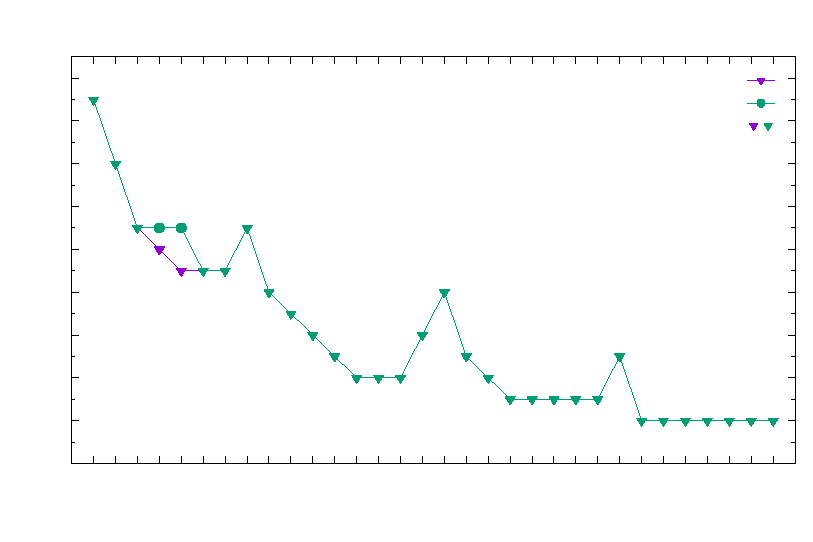
\includegraphics{resultados_3x3}}%
    \gplfronttext
  \end{picture}%
\endgroup
